\documentclass[8pt]{extarticle}
\title{}
\author{}
\date{}
\usepackage[shortlabels]{enumitem}


%paper setup
\usepackage{geometry}
\geometry{letterpaper, portrait, margin=1in}
\usepackage{fancyhdr}
% sans serif font:
\usepackage{cmbright}
%symbols
\usepackage{amsmath}
\usepackage{bigints}
\usepackage{amssymb}
\usepackage{amsthm}
\usepackage{mathtools}
\usepackage[hidelinks]{hyperref}
\usepackage{gensymb}
\usepackage{multirow,array}
\usepackage{multicol}

\newtheorem*{remark}{Remark}
\usepackage[T1]{fontenc}
\usepackage[utf8]{inputenc}

%chemistry stuff
%\usepackage[version=4]{mhchem}
%\usepackage{chemfig}

%plotting
\usepackage{pgfplots}
\usepackage{tikz}
\tikzset{middleweight/.style={pos = 0.5}}
\usetikzlibrary{decorations.markings}
%\tikzset{weight/.style={pos = 0.5, fill = white}}
%\tikzset{lateweight/.style={pos = 0.75, fill = white}}
%\tikzset{earlyweight/.style={pos = 0.25, fill=white}}

%\usepackage{natbib}

%graphics stuff
\usepackage{graphicx}
\graphicspath{ {./images/} }
\usepackage[style=numeric, backend=biber]{biblatex} % Use the numeric style for Vancouver
\addbibresource{the_bibliography.bib}
%code stuff
%when using minted, make sure to add the -shell-escape flag
%you can use lstlisting if you don't want to use minted
%\usepackage{minted}
%\usemintedstyle{pastie}
%\newminted[javacode]{java}{frame=lines,framesep=2mm,linenos=true,fontsize=\footnotesize,tabsize=3,autogobble,}
%\newminted[cppcode]{cpp}{frame=lines,framesep=2mm,linenos=true,fontsize=\footnotesize,tabsize=3,autogobble,}

%\usepackage{listings}
%\usepackage{color}
%\definecolor{dkgreen}{rgb}{0,0.6,0}
%\definecolor{gray}{rgb}{0.5,0.5,0.5}
%\definecolor{mauve}{rgb}{0.58,0,0.82}
%
%\lstset{frame=tb,
%	language=Java,
%	aboveskip=3mm,
%	belowskip=3mm,
%	showstringspaces=false,
%	columns=flexible,
%	basicstyle={\small\ttfamily},
%	numbers=none,
%	numberstyle=\tiny\color{gray},
%	keywordstyle=\color{blue},
%	commentstyle=\color{dkgreen},
%	stringstyle=\color{mauve},
%	breaklines=true,
%	breakatwhitespace=true,
%	tabsize=3
%}
% text + color boxes
\renewcommand{\mathbf}[1]{\mathbold{#1}}
\usepackage[most]{tcolorbox}
\tcbuselibrary{breakable}
\tcbuselibrary{skins}
\newtcolorbox{problem}[1]{colback=white,enhanced,title={\small #1},
          attach boxed title to top center=
{yshift=-\tcboxedtitleheight/2},
boxed title style={size=small,colback=black!60!white}, sharp corners, breakable}
%including PDFs
%\usepackage{pdfpages}
\setlength{\parindent}{0pt}
\usepackage{cancel}
\pagestyle{fancy}
\fancyhf{}
\rhead{Avinash Iyer}
\lhead{Math 212: Homework 8}
\newcommand{\card}{\text{card}}
\newcommand{\ran}{\text{ran}}
\newcommand{\N}{\mathbb{N}}
\newcommand{\Q}{\mathbb{Q}}
\newcommand{\Z}{\mathbb{Z}}
\newcommand{\R}{\mathbb{R}}
\begin{document}
\renewcommand{\arraystretch}{1.5}
  \begin{problem}{17.1}
    \begin{description}[font=\normalfont]
      \item[2:]
        \begin{align*}
          \begin{pmatrix}x(t)\\y(t)\end{pmatrix} &= 2\begin{pmatrix}\cos(t)\\\sin(t)\end{pmatrix}\tag*{$0\leq t\leq \pi/2$}
        \end{align*}
      \item[10:]
        \begin{align*}
          \begin{pmatrix}x(t)\\y(t)\\z(t)\end{pmatrix} &= \begin{pmatrix}5\\5t - 1\\2t+1\end{pmatrix}
        \end{align*}
      \item[22:]
        \begin{align*}
          \begin{pmatrix}x(t)\\y(t)\\z(t)\end{pmatrix} &= \begin{pmatrix}2\cos(t)\\2\sin(t)\\1\end{pmatrix}
        \end{align*}
      \item[40:]
        \begin{align*}
          \begin{pmatrix}x(t)\\y(t)\end{pmatrix} &= \begin{pmatrix}t^2\\t\end{pmatrix}\tag*{$1\leq t \leq 8$}
        \end{align*}
      \item[44:]
        \begin{align*}
          \begin{pmatrix}x(t)\\y(t)\\z(t)\end{pmatrix} &= \begin{pmatrix}t\\5\cos(t)\\5\sin(t)\end{pmatrix}
        \end{align*}
      \item[64:] $L_1$ and $L_2$ are the same line.
    \end{description}
  \end{problem}
  \begin{problem}{17.2}
    \begin{description}[font=\normalfont]
      \item[2:]
        \begin{align*}
          \vec{v}(t) &= \begin{pmatrix}6t\\2t\\-2t\end{pmatrix}\\
          \vec{a}(t) &= \begin{pmatrix}6\\2\\-2\end{pmatrix}
        \end{align*}
      \item[8:]
        \begin{align*}
          \vec{v}(t) &= \begin{pmatrix}-3\sin(3t)\\5\cos(5t)\end{pmatrix}\\
          \Vert\vec{v}(t)\Vert &= \sqrt{9\sin^2(3t) + 25\cos^2(5t)}
        \end{align*}
      \item[12:]
        \begin{align*}
          \vec{v}(t) &= \begin{pmatrix}3\sin(2t)\\-\sin(t)\\2t\end{pmatrix}\\
          \Vert\vec{v}(t)\Vert &= \sqrt{9\sin^2(2t) + \sin^2(t) + 4t^2}
        \end{align*}
      \item[14:]
        \begin{align*}
          \int_{0}^{2\pi}\sqrt{9\sin^2(3t) + 25\cos^2(5t)}dt &\approx 24.603
        \end{align*}
      \item[20:]
        \begin{align*}
          \vec{v}(t) &= \begin{pmatrix}-6t^2-3\\12t^2+6\\18t^2 + 9\end{pmatrix}\\
          \vec{a}(t) &= \begin{pmatrix}-12t\\24t\\36t\end{pmatrix}
        \end{align*}
      \item[24:]
        \begin{align*}
          \vec{v}(t) &= \begin{pmatrix}3t^2 - 12\\2t + 10\end{pmatrix}\\
          \shortintertext{so when $t = \pm 2$, the particle is moving parallel to the $x$-axis, and when $t = -5$, the particle is moving parallel to the $y$-axis. As $t \rightarrow +\infty$, $x,y \rightarrow +\infty$, while as $t\rightarrow-\infty$, $x\rightarrow -\infty$ and $y\rightarrow +\infty$}
        \end{align*}
      \item[28:]
        \begin{enumerate}[(a)]
          \item
            \begin{align*}
              (1+t) + (5+2t) + (-7+t) &= 1\\
              4t-1 &= 1\\
              t &= \frac{1}{2}\\
              \begin{pmatrix}x\\y\\t\end{pmatrix} &= \begin{pmatrix}\frac{3}{2}\\6\\\frac{13}{2}\end{pmatrix}
            \end{align*}
          \item
            \begin{align*}
              \Vert \vec{v}\Vert &= \sqrt{1 + 4 + 1}\\
                                 &= \sqrt{6}\text{ m/s}
            \end{align*}
        \end{enumerate}
      \item[44:] I don't know how to do this problem.
    \end{description}
  \end{problem}
  \begin{problem}{17.3}
    \begin{description}[font=\normalfont]
      \item[2:]
        \begin{align*}
          \vec{F}(x,y) &= \begin{pmatrix}-y\\0\end{pmatrix}
        \end{align*}
      \item[4:]
        \begin{align*}
          \vec{F}(x,y) &= \begin{pmatrix}-y\\x\end{pmatrix}
        \end{align*}
      \item[6:]
        \begin{align*}
          \vec{F}(x,y) &= \begin{pmatrix}x\\y\end{pmatrix}
        \end{align*}
      \item[8:] The vector field is neither parallel to the $x$-axis nor the $y$-axis. As $x$ increases, the length remains constant, while as $y$ increases, the length also increases.
      \item[10:] The vector field is neither parallel to the $x$-axis nor the $y$-axis. As $x$ increases and as $y$ increases, the length also increases.
      \item[24:]
        \begin{align*}
          \vec{F}(x,y) &= \begin{pmatrix}y\\y\end{pmatrix}
        \end{align*}
      \item[26:]
        \begin{align*}
          \vec{F}(x,y) &= \begin{pmatrix}x\\y\end{pmatrix}
        \end{align*}
      \item[28:]
        \begin{enumerate}[(I)]
          \item (C)
          \item (B)
          \item (A)
          \item (D)
        \end{enumerate}
      \item[32:]
        \begin{align*}
          \vec{F}(x,y) &= \begin{pmatrix}x\\0\end{pmatrix}
        \end{align*}
    \end{description}
  \end{problem}
  \begin{problem}{17.4}
    \begin{description}[font=\normalfont]
      \item[2:]\hfill
        \begin{center}
          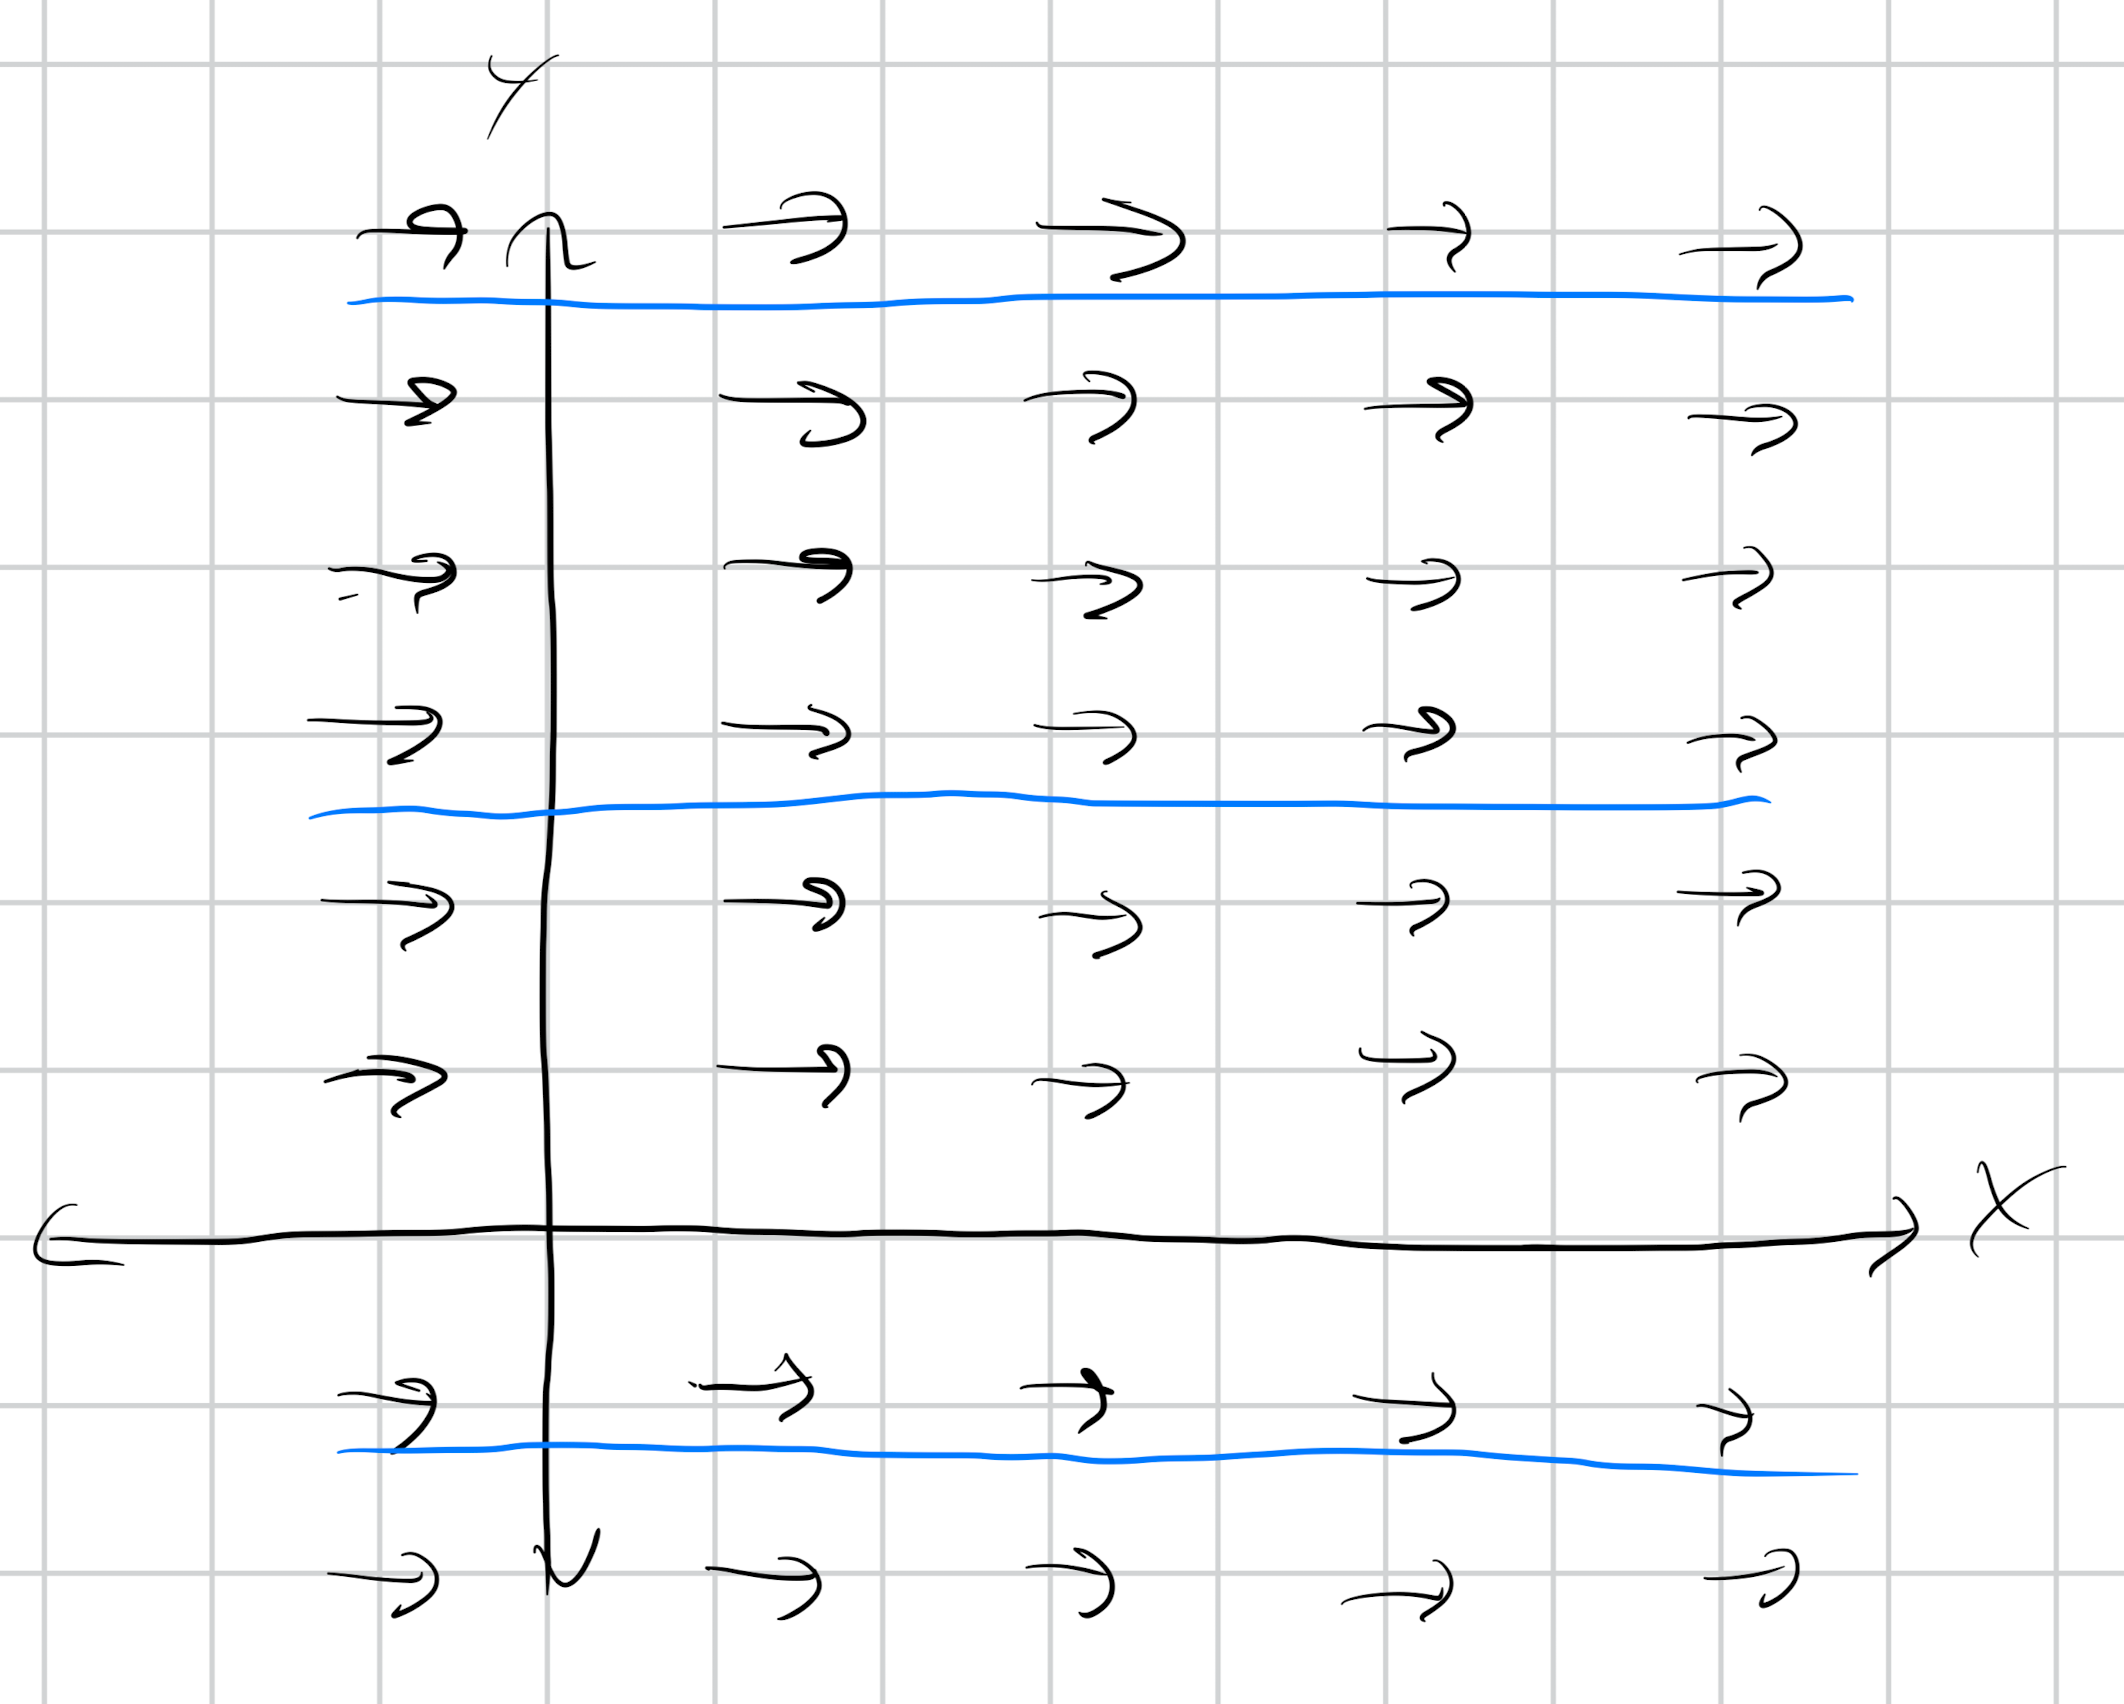
\includegraphics[width=10cm]{images/17_4_2.png}
        \end{center}
      \item[6:] \hfill
        \begin{center}
          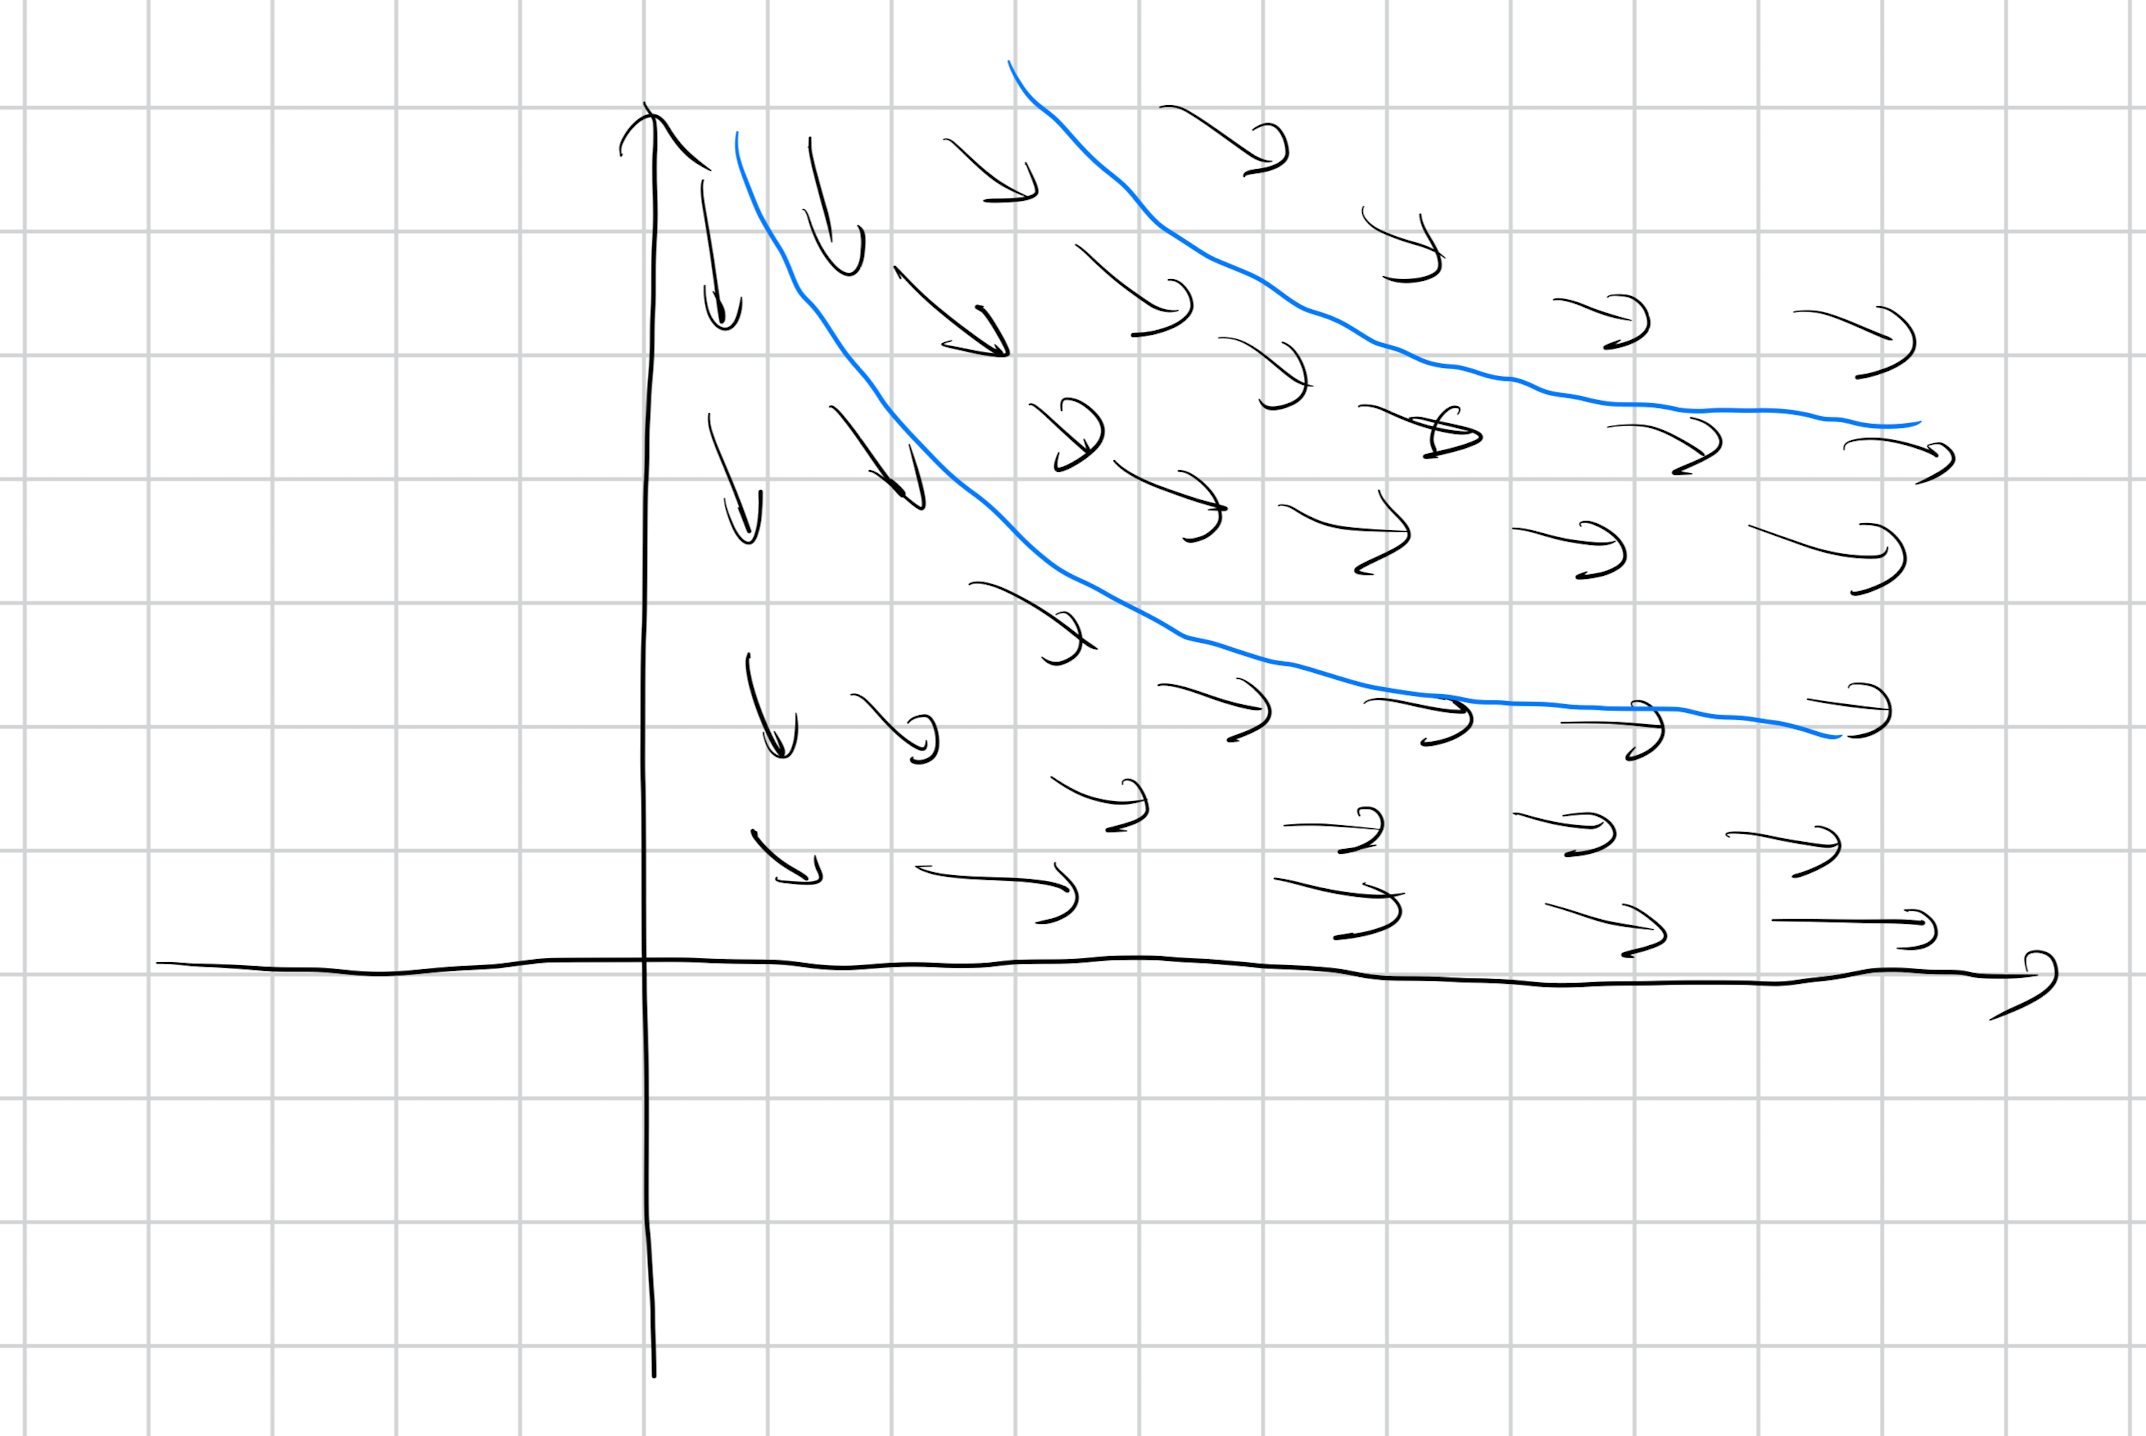
\includegraphics[width=10cm]{images/17_4_6.png}
        \end{center}
    \begin{align*}
      \begin{pmatrix}x'(t)\\y'(t)\end{pmatrix} &= \begin{pmatrix}x\\-y\end{pmatrix}\\
      x'(t) &= x(t)\\
      y'(t) &= -y(t)\\
      x'(t) &= x_0e^{t}\\
      y'(t) &= y_0e^{-t}
    \end{align*}
      \item[8:]\hfill
        \begin{center}
          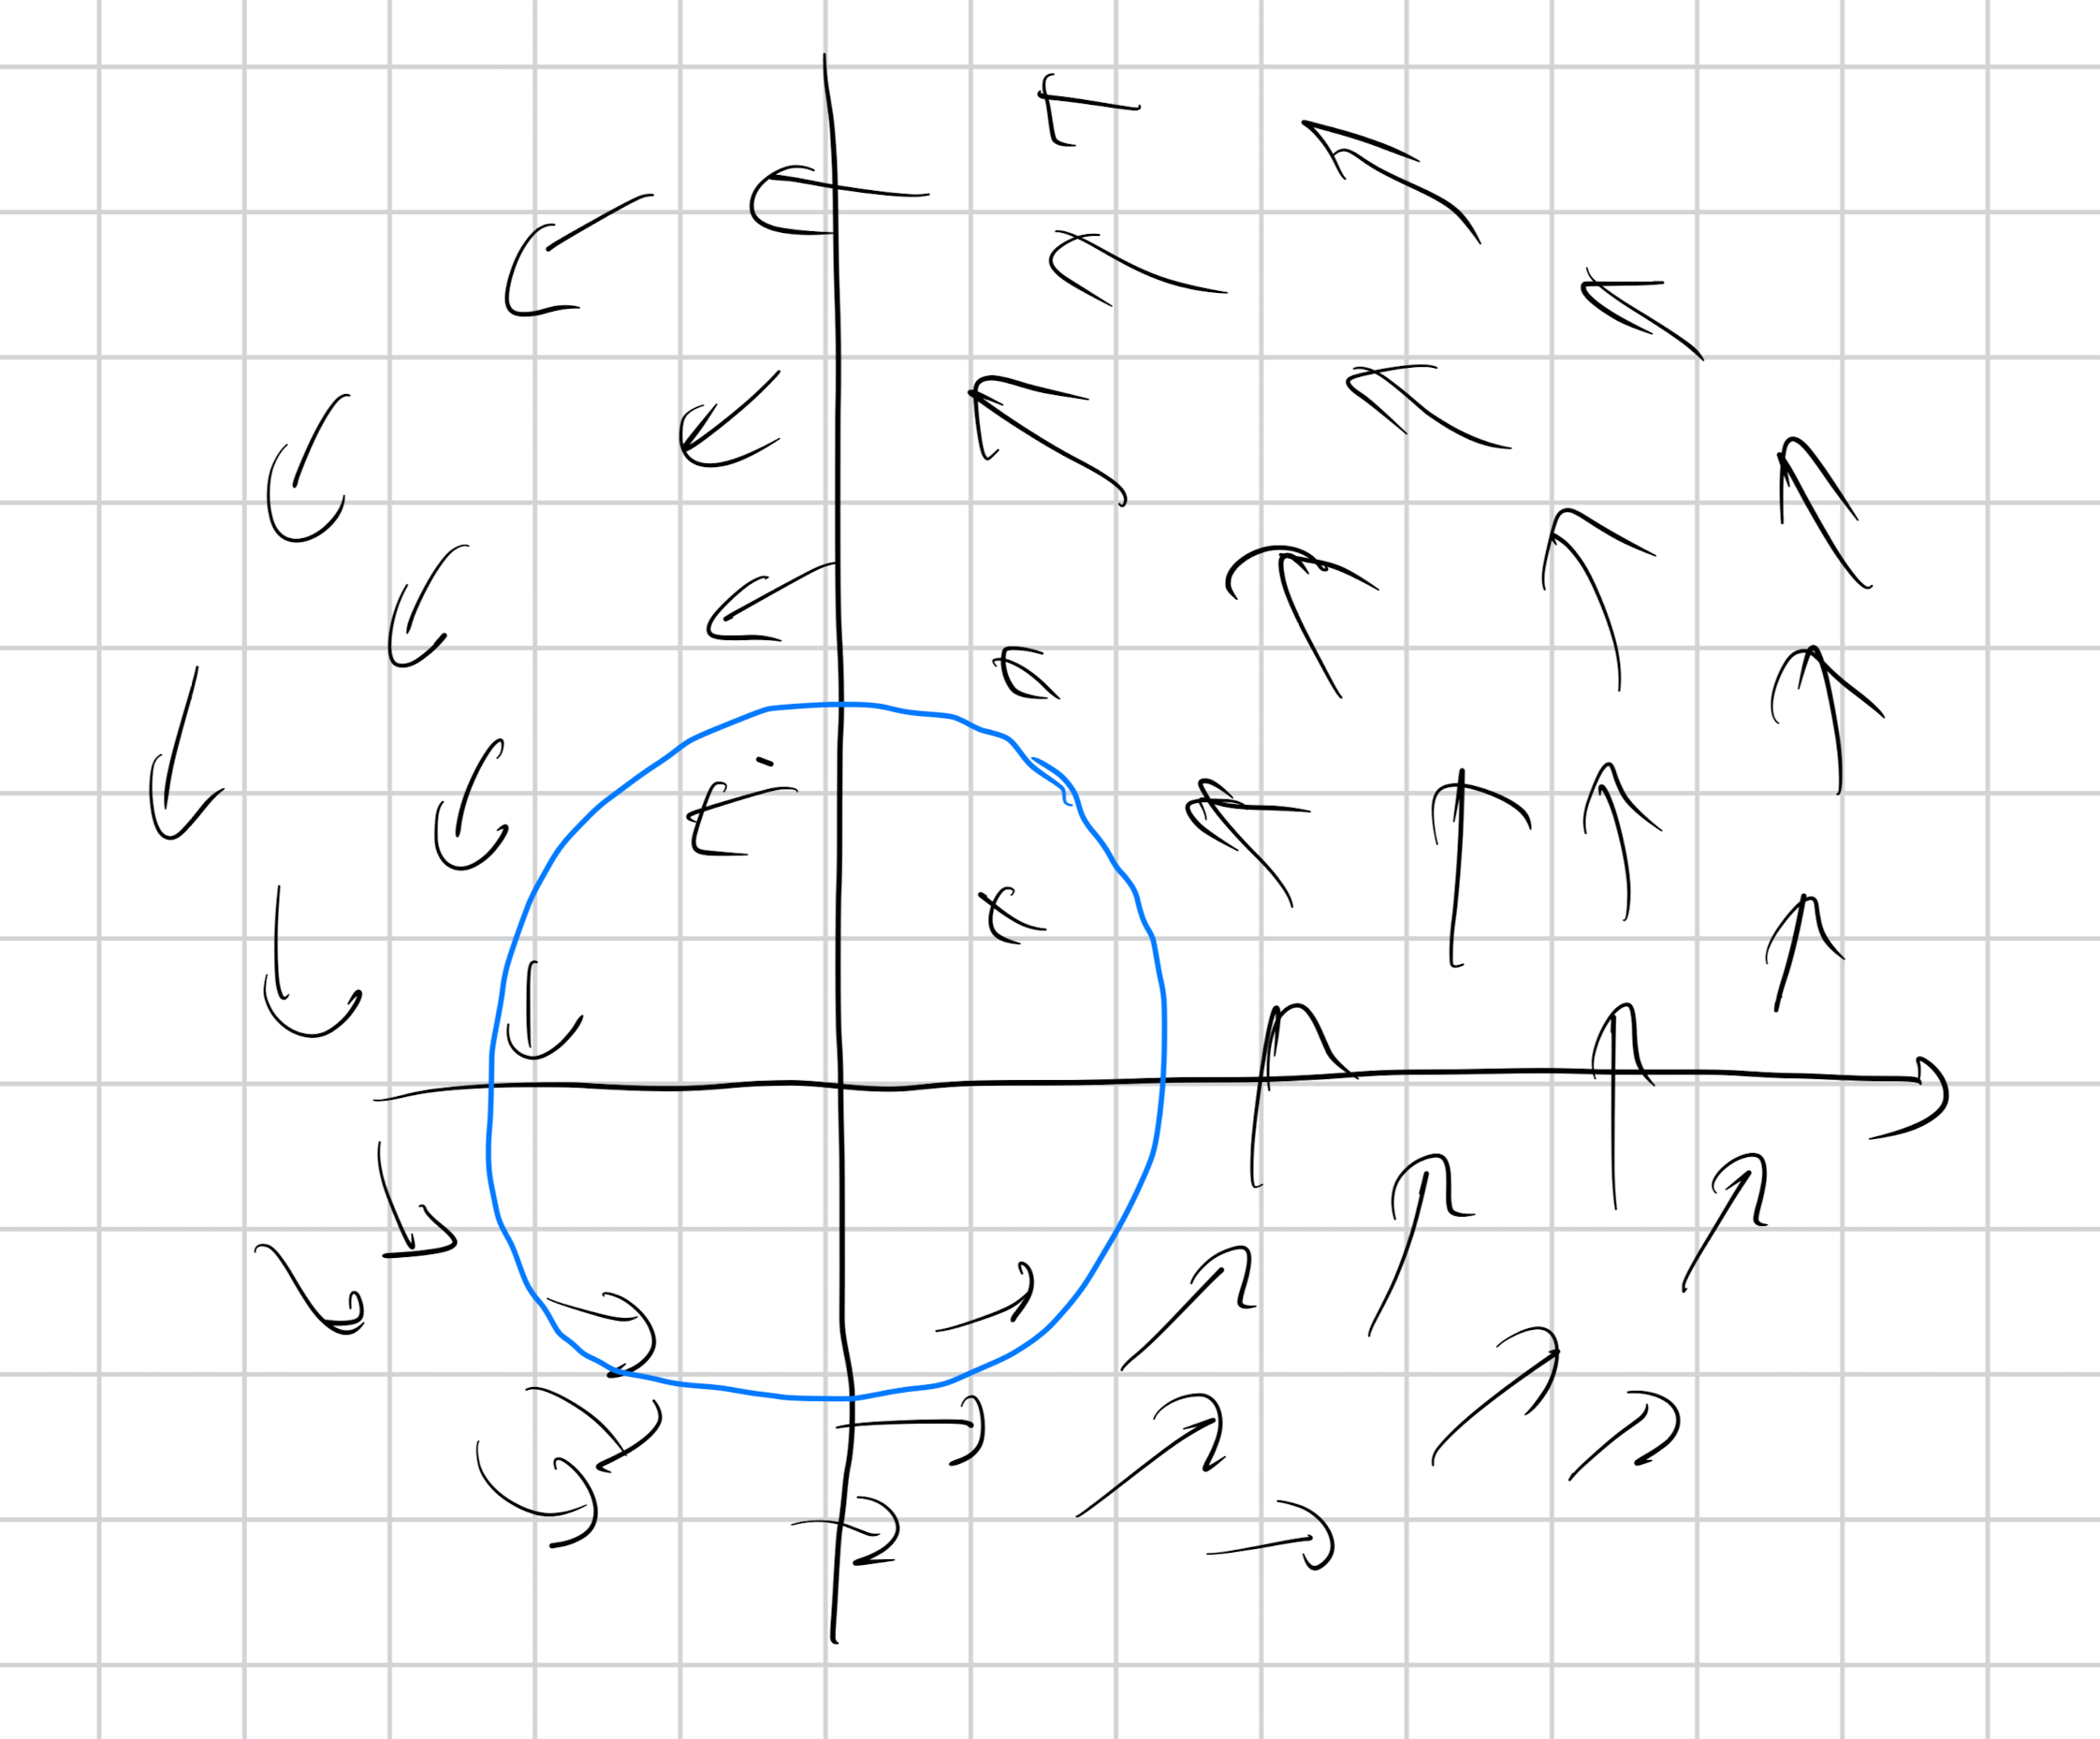
\includegraphics[width=10cm]{images/17_4_8.png}
        \end{center}
      \item[16:]\hfill
        \begin{enumerate}[(a)]
          \item (III)
          \item (I)
          \item (II)
          \item (V)
          \item (VI)
          \item (IV)
        \end{enumerate}
      \item[20:]
        \begin{align*}
          \begin{pmatrix}x'(t)\\y'(t)\end{pmatrix}&= \begin{pmatrix}x\\-y\end{pmatrix}\\
          \nabla f &= \begin{pmatrix}2x\\-2y\end{pmatrix}\\
          \begin{pmatrix}x'(t)\\y'(t)\end{pmatrix}&= \frac{1}{2}\nabla f
        \end{align*}
    \end{description}
  \end{problem}
\end{document}
